\documentclass{article}
\usepackage{graphicx}
\usepackage{hyperref}
\usepackage{tablefootnote}


\renewcommand{\figurename}{Figura}
\renewcommand{\tablename}{Tabella}

\title{Report di Laboratorio di Making}
\author{Daniele Romanella - daniele.romanella@studio.unibo.it - 0001170158}
\date{22 luglio 2025}

\begin{document}

\maketitle


\section{Introduzione}
Il progetto prevede la realizzazione di un veicolo telecomandato tramite smartphone, utilizzando una connessione Bluetooth e un'applicazione dedicata. A differenza delle tradizionali auto giocattolo, il sistema proposto è concepito come una piattaforma espandibile in pochi passi, consentendo l'integrazione di funzionalità avanzate e personalizzabili (i.e. Computer Vision, guida autonoma, etc.), ampliando così le potenzialità d’uso.

\subsection{Risultati}
Nelle \textbf{figure 1, 2, 3} e \textbf{4} sono rappresentati rispettivamente i risultati del progetto: la macchina con la carrozzeria montata (vista frontale), la macchina con la carrozzeria montata (vista posteriore), la struttura senza carrozzeria e l'interfaccia dell'applicazione per il controllo tramite smartphone.

\begin{figure}[h!]
  \centering
  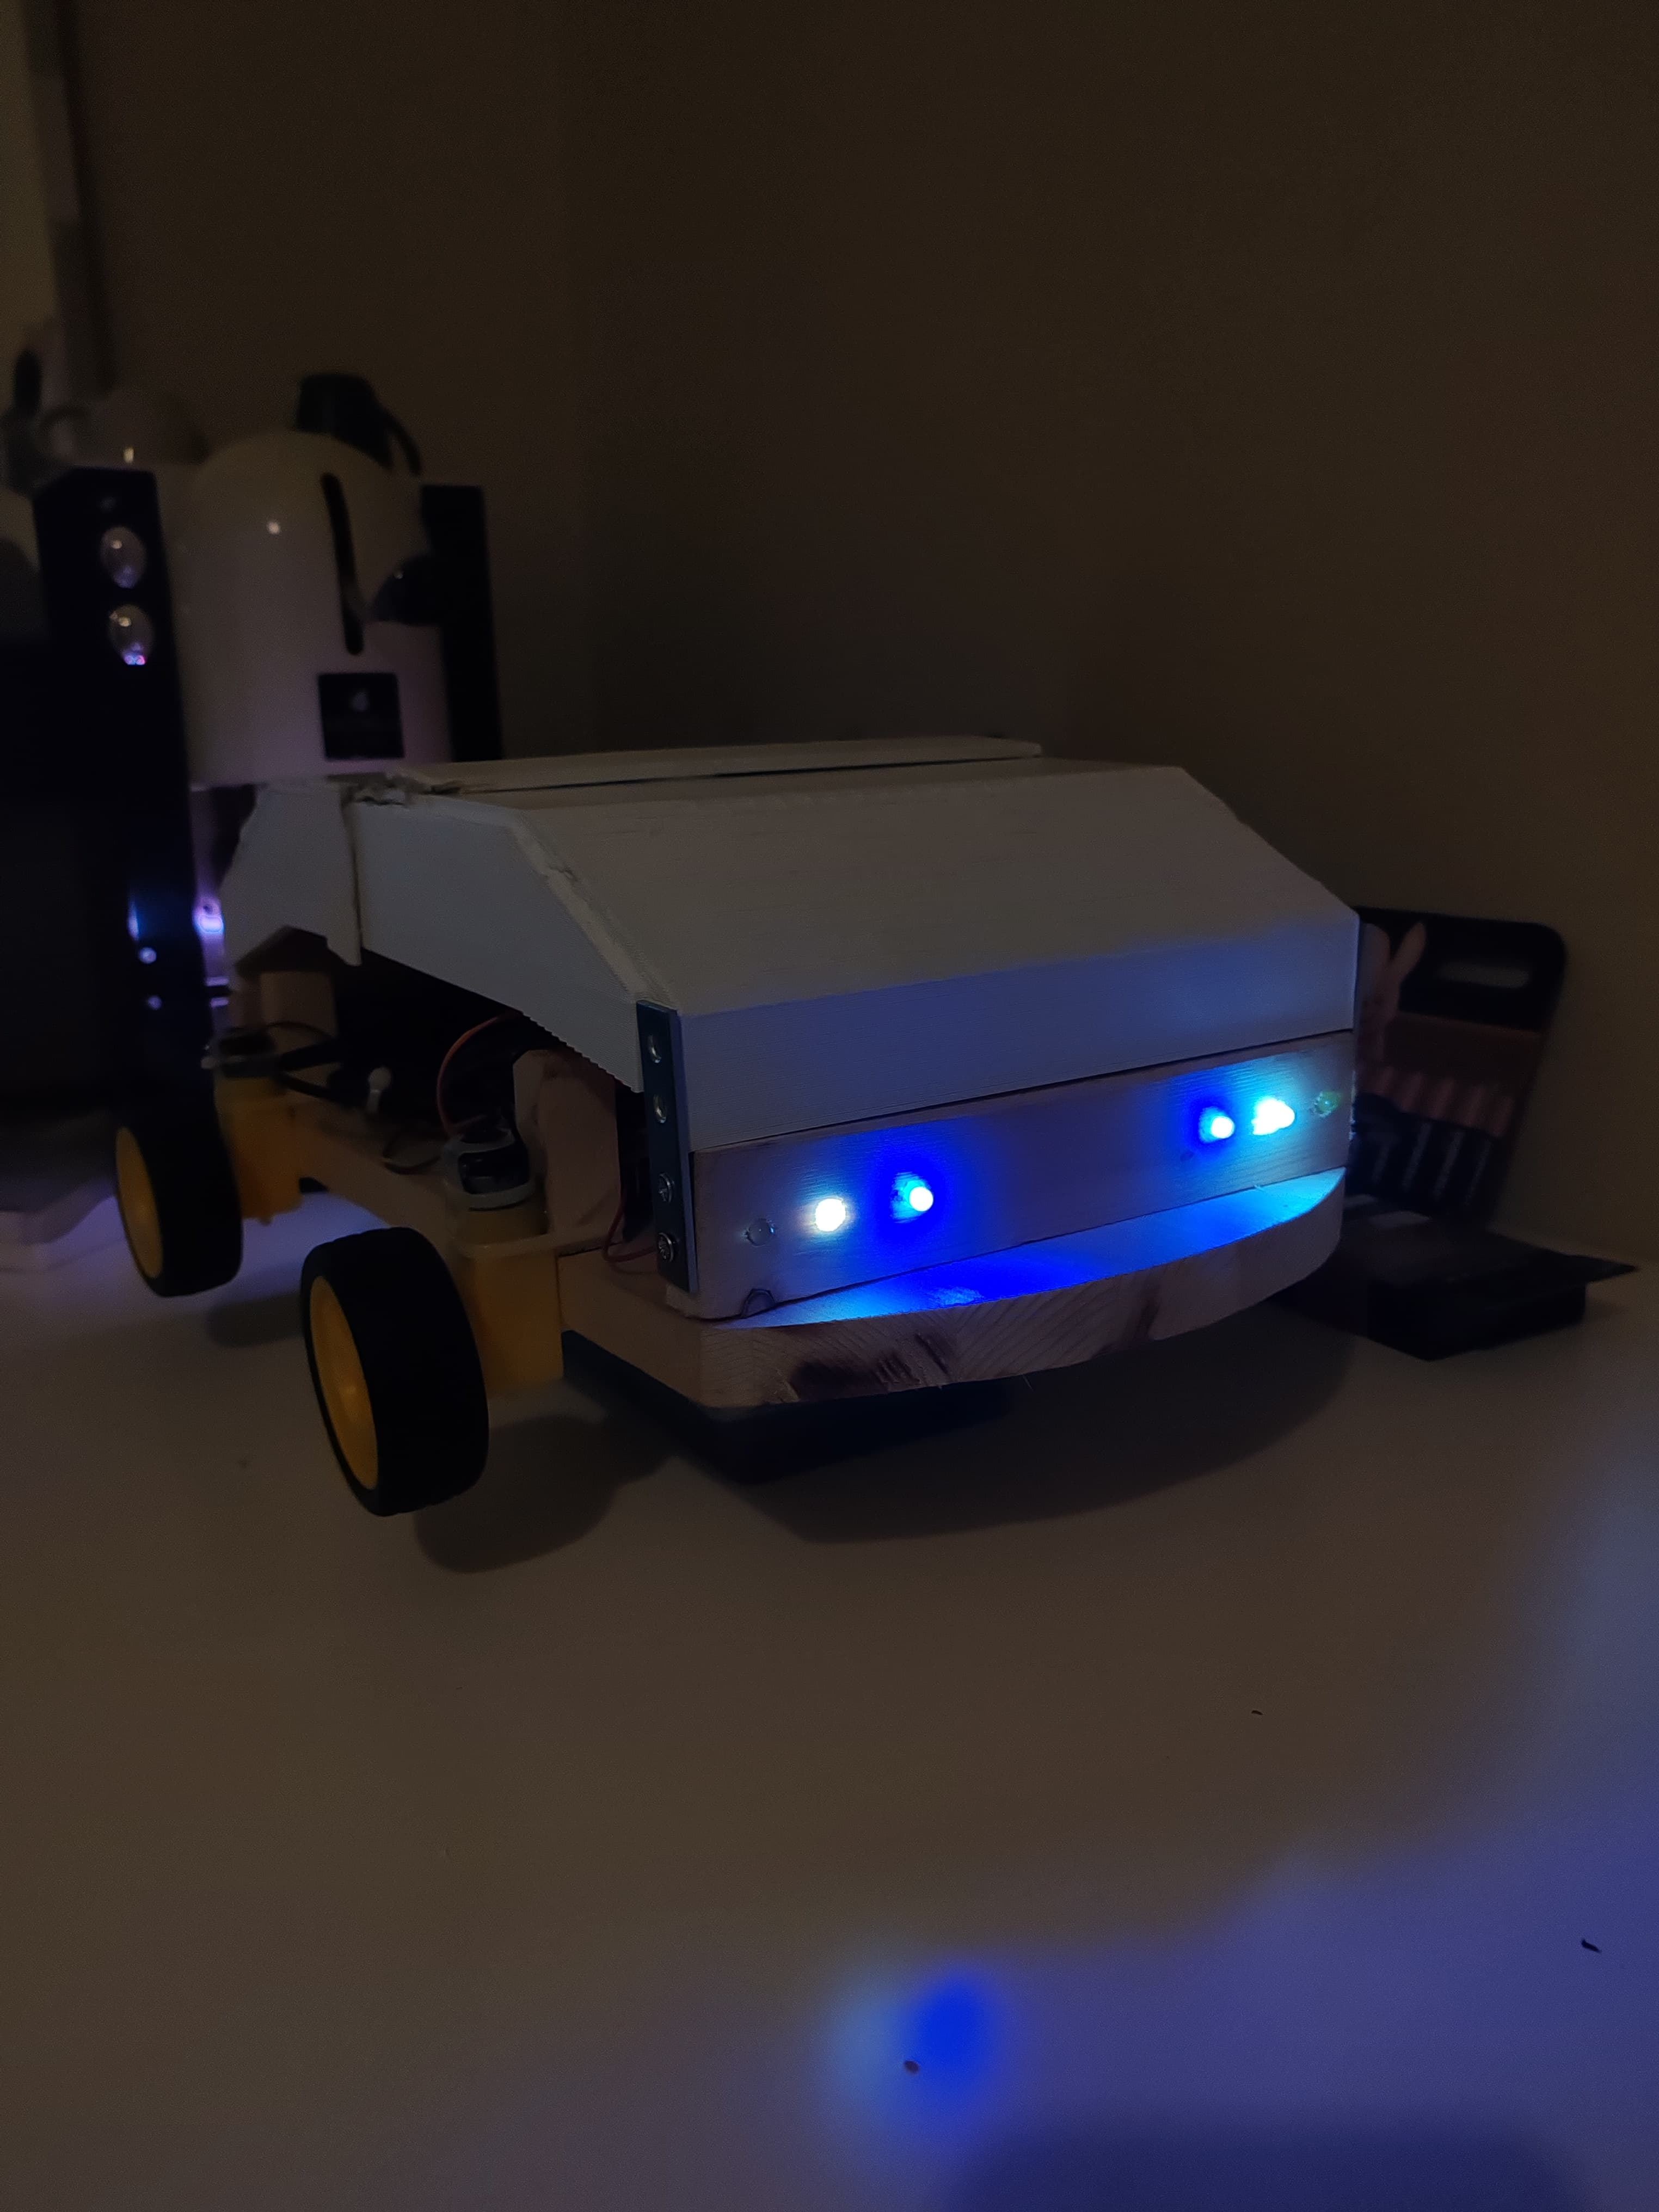
\includegraphics[width=0.5\textwidth]{imgs/results_1.jpeg}
  \caption{La macchina con la carrozzeria montata. (vista frontale)}
  \label{fig:macchina_carrozzeria}
\end{figure}

\begin{figure}[h!]
  \centering
  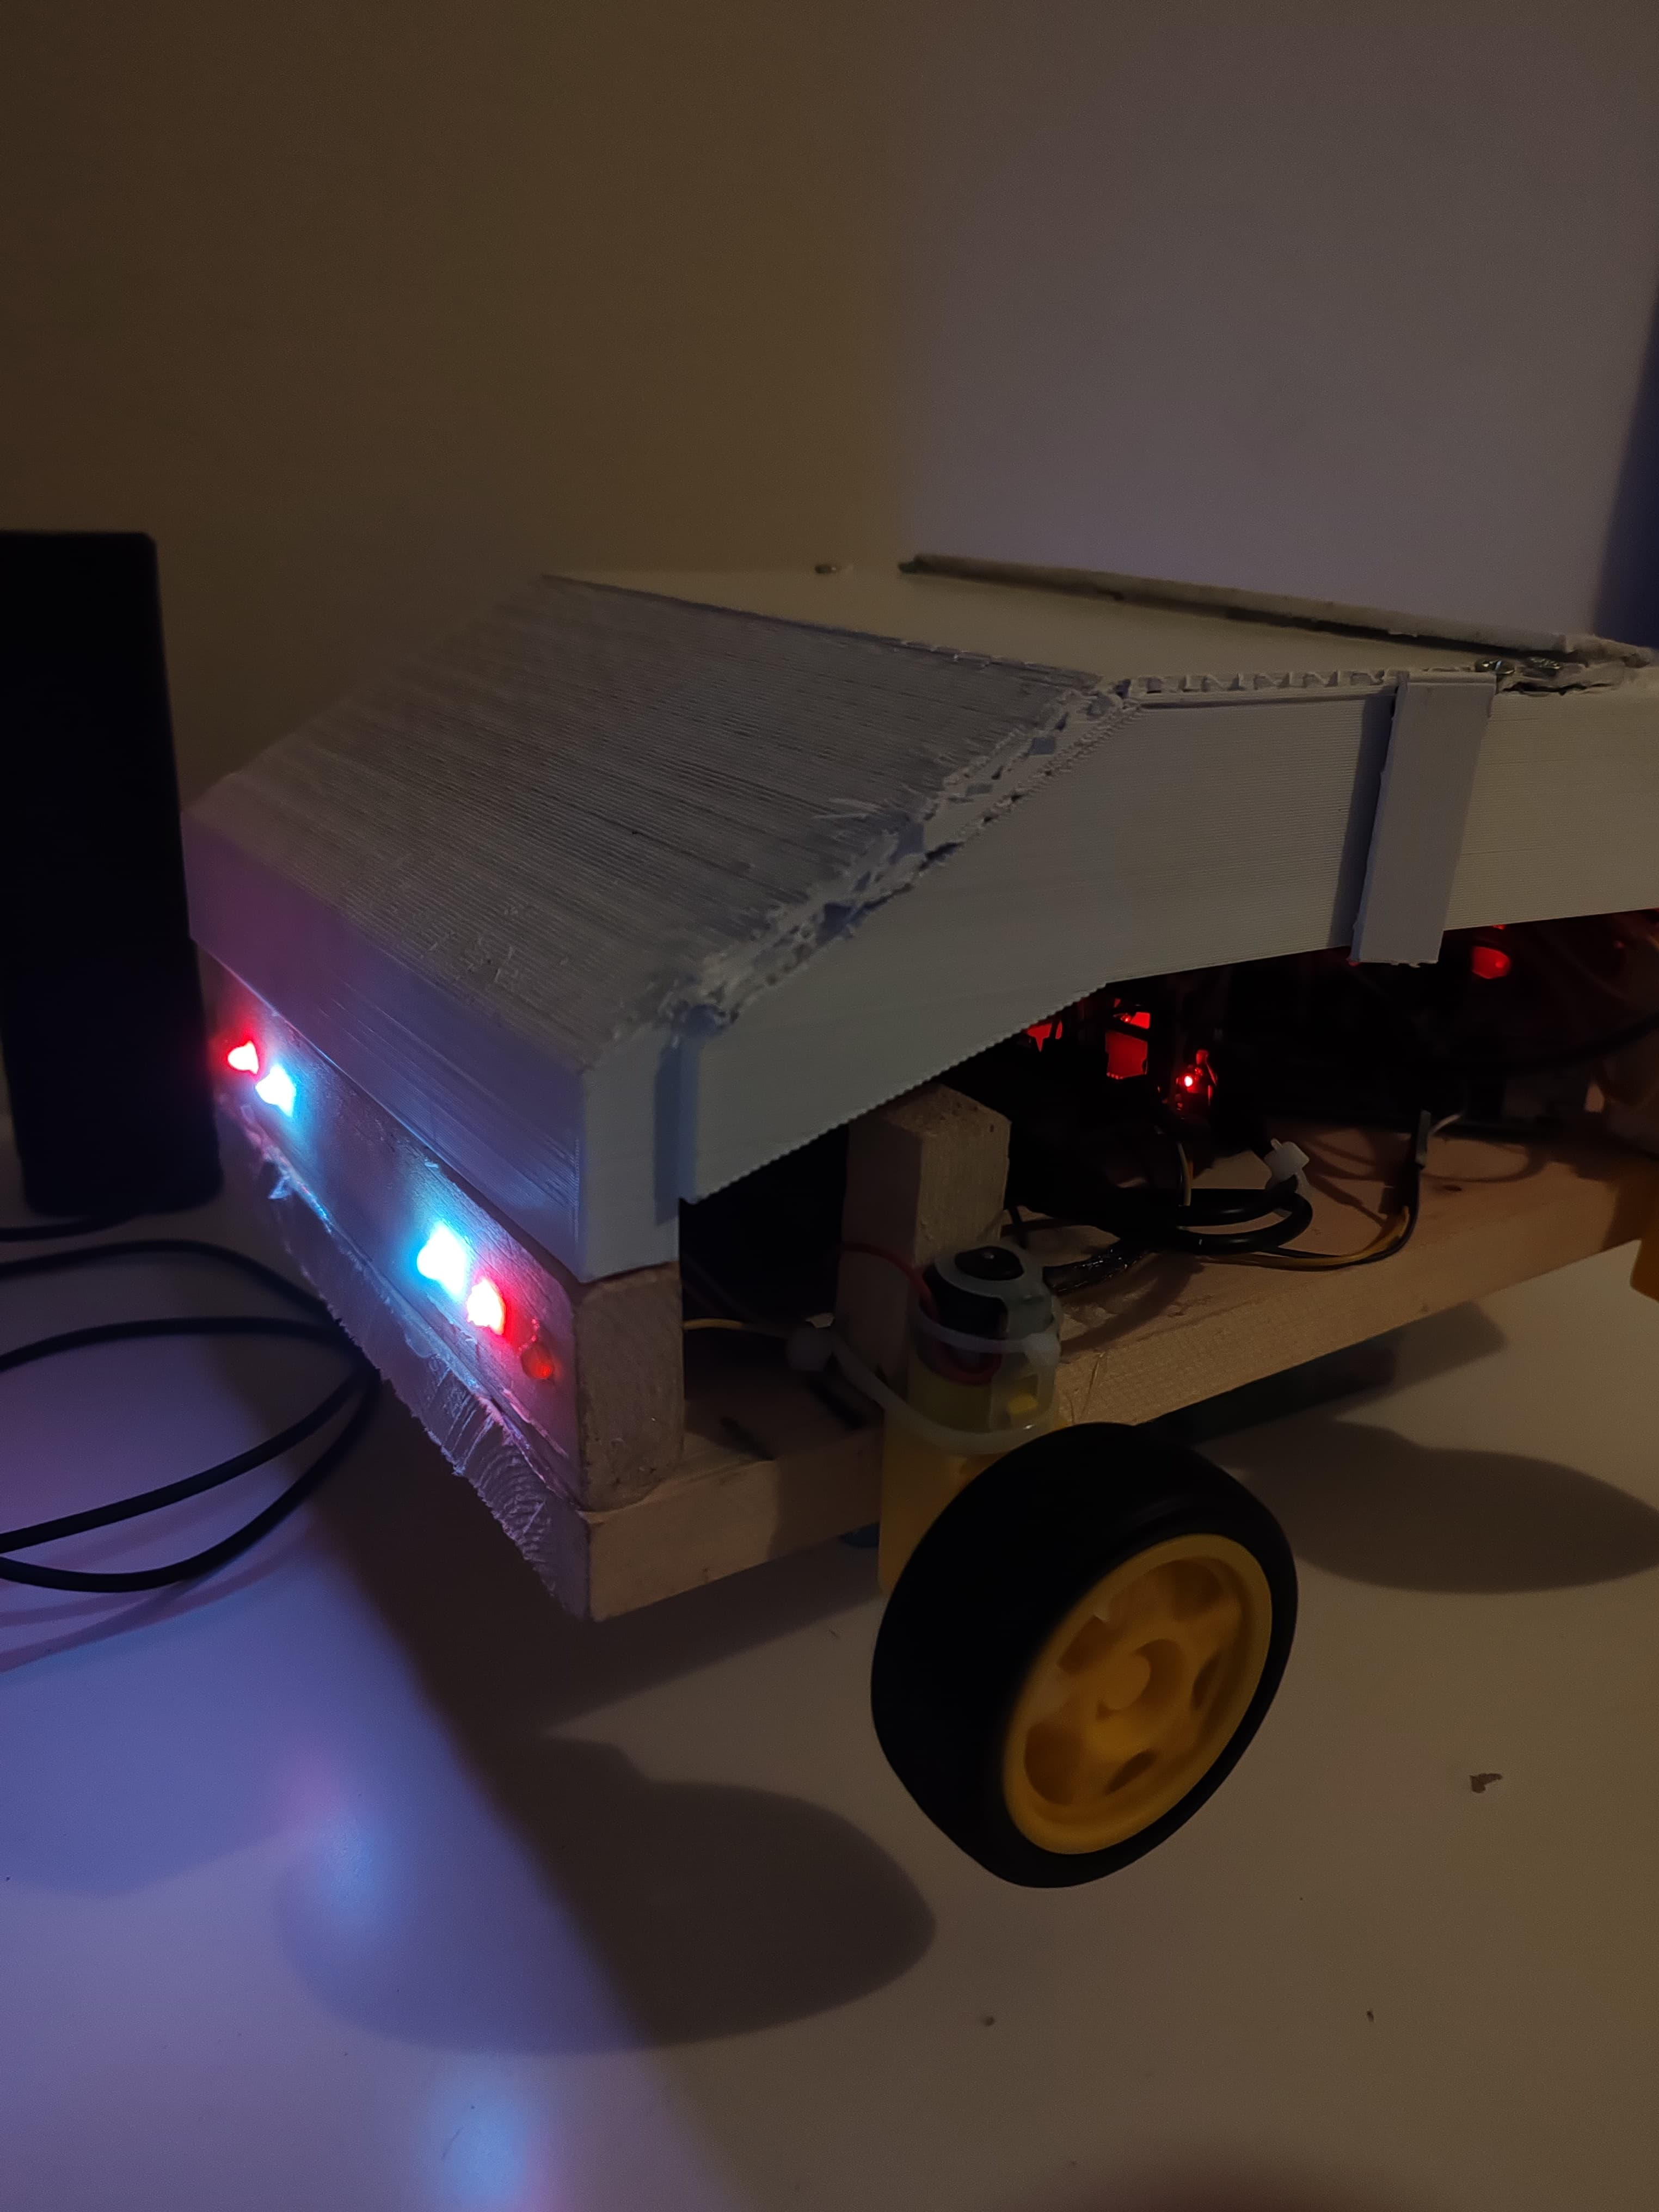
\includegraphics[width=0.5\textwidth]{imgs/results_2.jpeg}
  \caption{La macchina con la carrozzeria montata. (vista posteriore)}
  \label{fig:macchina_carrozzeria}
\end{figure}

\begin{figure}[h!]
  \centering
  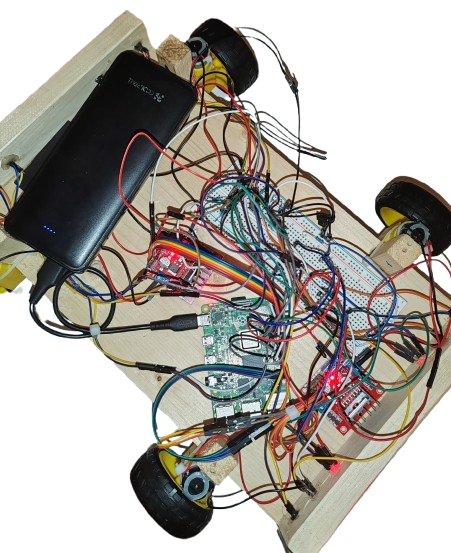
\includegraphics[width=0.5\textwidth]{imgs/results_3.png}
  \caption{La macchina senza carrozzeria.}
  \label{fig:macchina_carrozzeria}
\end{figure}

\begin{figure}[h!]
  \centering
  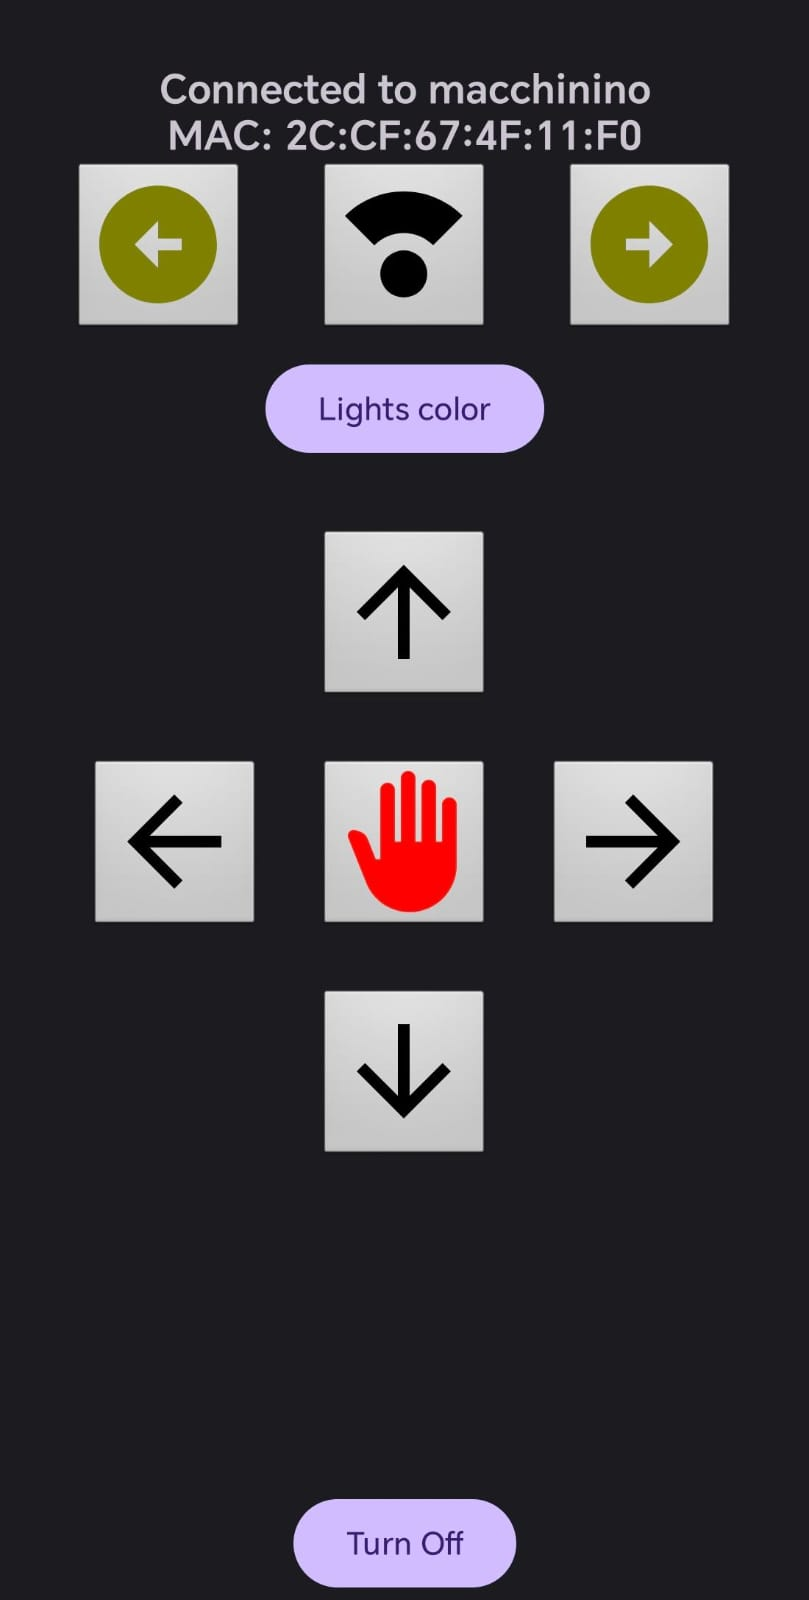
\includegraphics[width=0.25\textwidth]{imgs/results_4.jpeg}
  \caption{Applicazione android per controllare il progetto}
  \label{fig:macchina_carrozzeria}
\end{figure}

\newpage
\section{Costi ed Analisi di mercato}
Il costo complessivo sostenuto per la realizzazione del progetto ammonta a 62,62€. Tuttavia, sarebbe stato possibile contenere ulteriormente la spesa ricorrendo a fornitori con tempi di consegna più lunghi: in tal caso, il costo minimo teoricamente raggiungibile, considerando esclusivamente prezzi al dettaglio e l'acquisto di tutti i componenti ex novo, sarebbe stato pari a 55,41€.
\newline
Per quanto riguarda i prodotti concorrenti, i prototipi in grado di offrire funzionalità analoghe — ovvero veicoli controllabili via Bluetooth — presentano generalmente un costo elevato e una reperibilità limitata sul mercato. Il presente progetto si distingue non solo per il costo contenuto, ma anche per la possibilità di effettuare il deployment di applicazioni aggiuntive, come algoritmi di visione artificiale, grazie all'integrazione di una Pi Camera.

Nel confronto con le comuni auto giocattolo telecomandate, il prototipo sviluppato risulta più costoso; tuttavia, offre funzionalità avanzate generalmente assenti nei prodotti commerciali, come il controllo individuale delle luci.

Il target di riferimento è duplice: da un lato, si rivolge a utenti esperti e appassionati di tecnologie embedded, che ricercano una piattaforma flessibile per sperimentazioni avanzate (es. computer vision, guida autonoma); dall’altro, il dispositivo risulta facilmente utilizzabile anche da un pubblico non esperto, in quanto il sistema è perfettamente operativo dopo il semplice abbinamento Bluetooth, senza necessità di ulteriori configurazioni.
\subsection{Materiale usato}
La \textbf{Tabella 1} riporta i materiali impiegati nel progetto. Quando compatibile, alcuni componenti sono stati riutilizzati da precedenti realizzazioni, con l’obiettivo di ottimizzare l’utilizzo delle risorse. Nel presente report non sono stati considerati i costi di ammortamento degli strumenti impiegati, assumendo per semplicità una disponibilità illimitata degli stessi.
\begin{table}[h!]
\centering
\begin{tabular}{|c|c|c|}
\hline
\textbf{Componente} & \textbf{Prezzo} & \textbf{Provenienza} \\
\hline
Raspberry Pi 4 (4 GB) & Riutilizzato & - \\
Legno per pianale (20 mm) & 5€ & Negozio di fai da te \\
Led, breadboard e cavi & 19,99€ & \href{https://www.amazon.it/dp/B01MQIO78W}{Amazon.it} \\
Motori (6V) e ruote & 12,99€ & \href{https://www.amazon.it/dp/B096Z5C3R4}{Amazon.it} \\
L298N & 3,49€ (x 2) & \href{https://www.amazon.it/dp/B08K3886W7}{Amazon.it} \\
Portabatterie & 1,33€ (x 2) & \href{https://www.amazon.it/dp/B07WJ3HFSP}{Amazon.it} \\
Powerbank & Riutilizzato & - \\
Stampa carrozzeria superiore & 15€ & - \\
Scheda SD & Riutilizzato & - \\
\hline
\end{tabular}
\caption{Tabella dei componenti con prezzo e provenienza.}
\label{tab:componenti}
\end{table}
\subsection{Possibili ottimizzazioni}
I materiali elencati nella \textbf{Tabella 1} sono stati selezionati in base al buon rapporto qualità-prezzo e alla loro pronta disponibilità. La \textbf{Tabella 2}, invece, riporta alternative a costo inferiore, ma caratterizzate da tempi di approvvigionamento più lunghi, oppure da materiale che offre meno performance ma che sarebbe più indicato per questo scopo.
\begin{table}[h]
\centering
\begin{tabular}{|c|c|c|c|c|}
\hline
\textbf{Componente} & \textbf{Prezzo} & \textbf{Risparmio} & \textbf{Provenienza} \\
\hline
Raspberry Pi Zero 2W\tablefootnote{Richiede saldatura degli headers} & 21,59€ & -  &  \href{https://it.aliexpress.com/item/1005006143379283.html}{AliExpress}\\
Headers da saldare & 0,87€ & -  &  \href{https://it.aliexpress.com/item/1005003723352206.html}{AliExpress}\\
Legno per pianale (20 mm) & 1,50€ & 3,50€ & Negozio di fai da te \\
Led, breadboard e cavi & 10,88€ & 9,11€ & \href{https://www.temu.com/it-en/beginners-starter-kit-830pcs-electronic-components-set-with-breadboard-sensors-leds-for-diy-electronics-projects-g-601101343933992.html}{TEMU}\tablefootnote{\`E stato cercato un kit che comprendesse due LED RGB, esattamente come nel progetto. Una variazione sarebbe quella di usare dei led non RGB per risparmiare ulteriormente} \\
Motori (6V) e ruote & 0,87€ (x 2) & 11,25€ & \href{https://it.aliexpress.com/item/1005005699364066.html}{AliExpress} \\
L298N & 0,87€ (x 2) & 5,24€ & \href{http://it.aliexpress.com/item/32392774289.html}{AliExpress} \\
Portabatterie & 1,98€ & 0,68€ & \href{https://www.amazon.it/dp/B07WJ3HFSP}{Amazon.it} \\
Powerbank & 9,24€ & - & \href{https://www.temu.com/it-en/20000mah-portable-charging-treasure-mobile-phone-battery-pack-22w-fast-charger-with--display-usb-type-c-micro-interface-suitable-for-iphone--phone-electronic-equipment-gift-outdoor-emergency-power-backup-battery-pack-g-601099542276300.html}{Temu} \\
Stampa carrozzeria superiore \tablefootnote{Rendendo alcune parti meno spesse.} & 5€ & 10€ & Prodotta in autonomia \\
Scheda SD (64 GB)\tablefootnote{Al momento della redazione di questo documento i tagli da 8GB, 16GB, 32GB e 64GB hanno lo stesso importo.} & 0,87€ & - & \href{https://it.aliexpress.com/item/1005006826605453.html}{AliExpress} \\
\hline
\end{tabular}
\caption{Tabella dei componenti con prezzo e provenienza.}
\label{tab:componenti}
\end{table}

\section{Implementazione hardware}
In questa sezione viene descritta l’implementazione hardware del progetto. Le sottosezioni successive approfondiscono la realizzazione del pianale, della carrozzeria e l’integrazione dei componenti elettronici.
\subsection{Pianale}
Il pianale inferiore presenta una lunghezza di 37cm, una larghezza di 19cm e uno spessore di 20mm. La sagoma è stata realizzata mediante taglio manuale con seghetto per legno. La curvatura frontale è stata ottenuta utilizzando un utensile flessibile dotato di disco abrasivo, lo stesso impiegato anche per la levigatura della superficie. Tale operazione ha permesso di ottenere una finitura più liscia, riducendo il rischio di schegge e migliorando la maneggevolezza del componente.
\subsubsection{Alloggio luci}
Gli alloggiamenti per i LED sono stati ricavati da una porzione residua della tavola di legno utilizzata per il pianale. Ogni alloggio misura 15mm di lunghezza, 19cm di larghezza e 35mm di altezza. Sono presenti fori per l’inserimento dei LED, realizzati con trapano e punta da 5mm di diametro. I LED sono stati posizionati all’interno dei fori e fissati mediante colla a caldo; successivamente sono stati collegati i cavi necessari per il cablaggio e l’integrazione con il circuito di controllo.
\subsubsection{Componenti di supporto per i motori}
I supporti destinati al fissaggio dei motori presentano una lunghezza e una larghezza di 20mm, con un’altezza pari a 5cm. Essi sono stati montati sulla base del veicolo mediante una vite. Il foro necessario per l'inserimento della vite è stato realizzato con l’ausilio di un trapano, utilizzando una punta da 7mm di diametro.
\newline
I motori sono stati ancorati ai supporti tramite l’utilizzo della colla a caldo e una fascetta in plastica (fascetta da elettricista), garantendo un montaggio stabile.
\subsection{Carrozzeria}

La carrozzeria del veicolo è stata realizzata tramite stampa 3D. Sono stati sviluppati due progetti distinti:

\begin{itemize}
    \item \textbf{Il primo progetto}, effettivamente stampato e implementato, presenta diverse criticità legate a una progettazione non ottimale. È visibile nella \textbf{figura 1} e nella \textbf{figura 2}.

    \item \textbf{Il secondo progetto}, considerato definitivo, non è stato stampato a causa dell’eccessivo peso che avrebbe comportato e degli elevati costi di stampa. Una trattazione più approfondita di tali problematiche è riportata nella sezione \textit{Problematiche}. Il modello relativo è illustrato nella \textbf{Figura 5} e nella \textbf{Figura 6}.
\end{itemize}

\begin{figure}
    \centering
    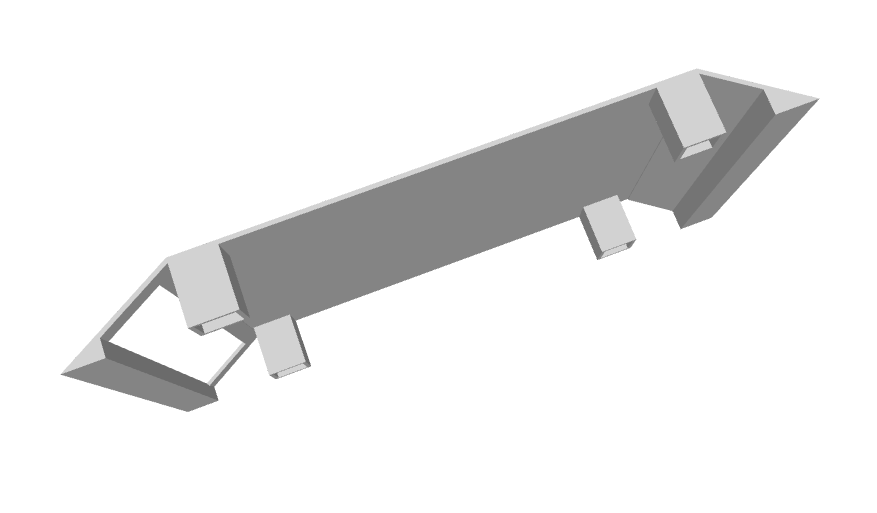
\includegraphics[width=0.5\linewidth]{imgs/carrozzeria_final.png}
    \caption{Carrozzeria finale, vista laterale. (Progetto)}
    \label{fig:enter-label}
\end{figure}
\begin{figure}
    \centering
    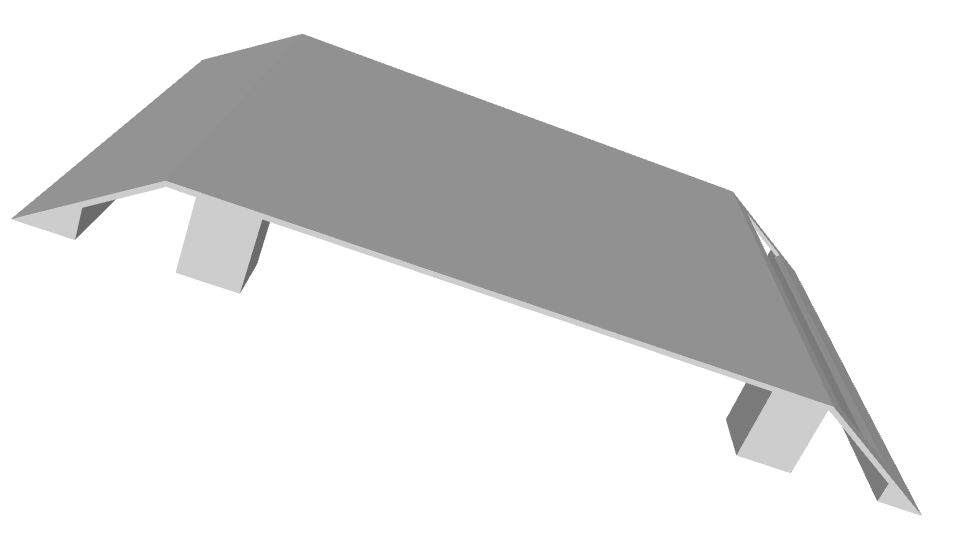
\includegraphics[width=0.5\linewidth]{imgs/carrozzeria_final_2.png}
    \caption{Carrozzeria finale, vista superiore. (Progetto)}
    \label{fig:enter-label}
\end{figure}
\subsection{Circuito}
L'implementazione del circuito deve rispettare i seguenti diagrammi Fritzing: Uno per i motori ed uno per le luci.
\newline
Nei circuiti si fa notare che i motori hanno un voltaggio di 6V. Per quanto riguarda le luci RGB del tipo \textit{Common anode}.
Le immagini dei circuiti sono in \textbf{Figura 7} e in \textbf{Figura 8}.
\begin{figure}
    \centering
    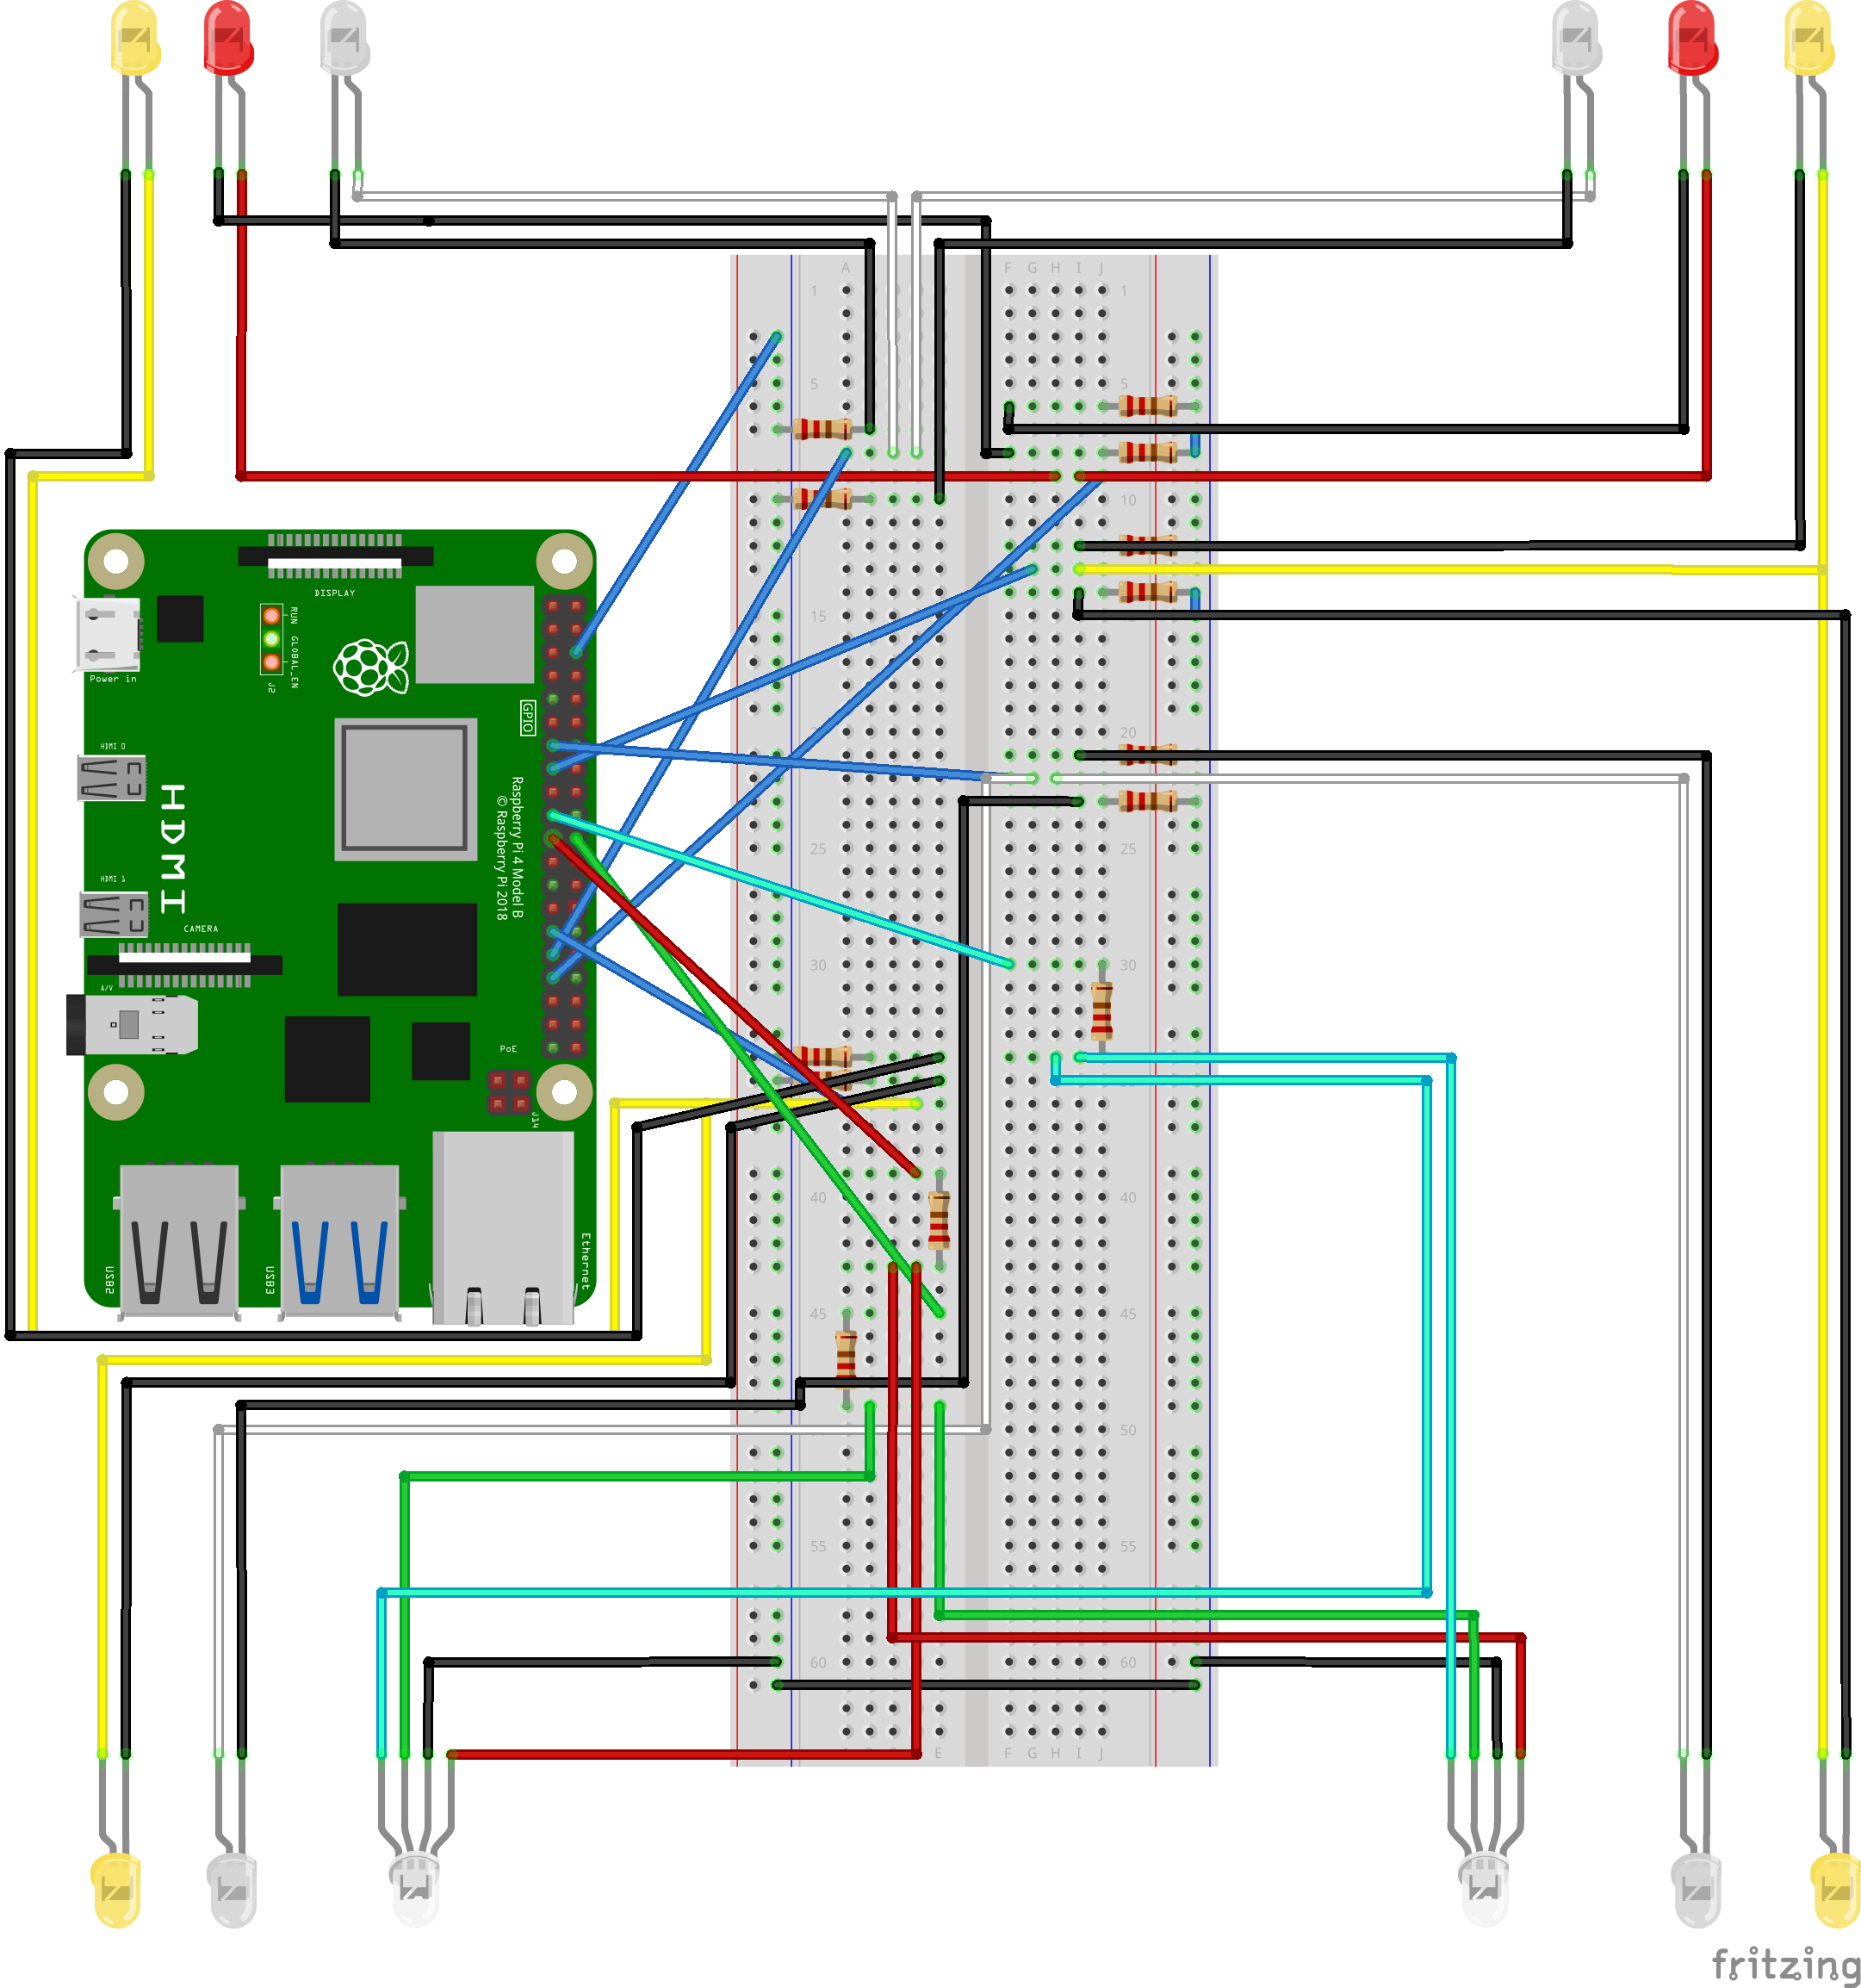
\includegraphics[width=0.5\linewidth]{imgs/luci.png}
    \caption{Circuito relativo alle luci.}
    \label{fig:enter-label}
\end{figure}
\begin{figure}
    \centering
    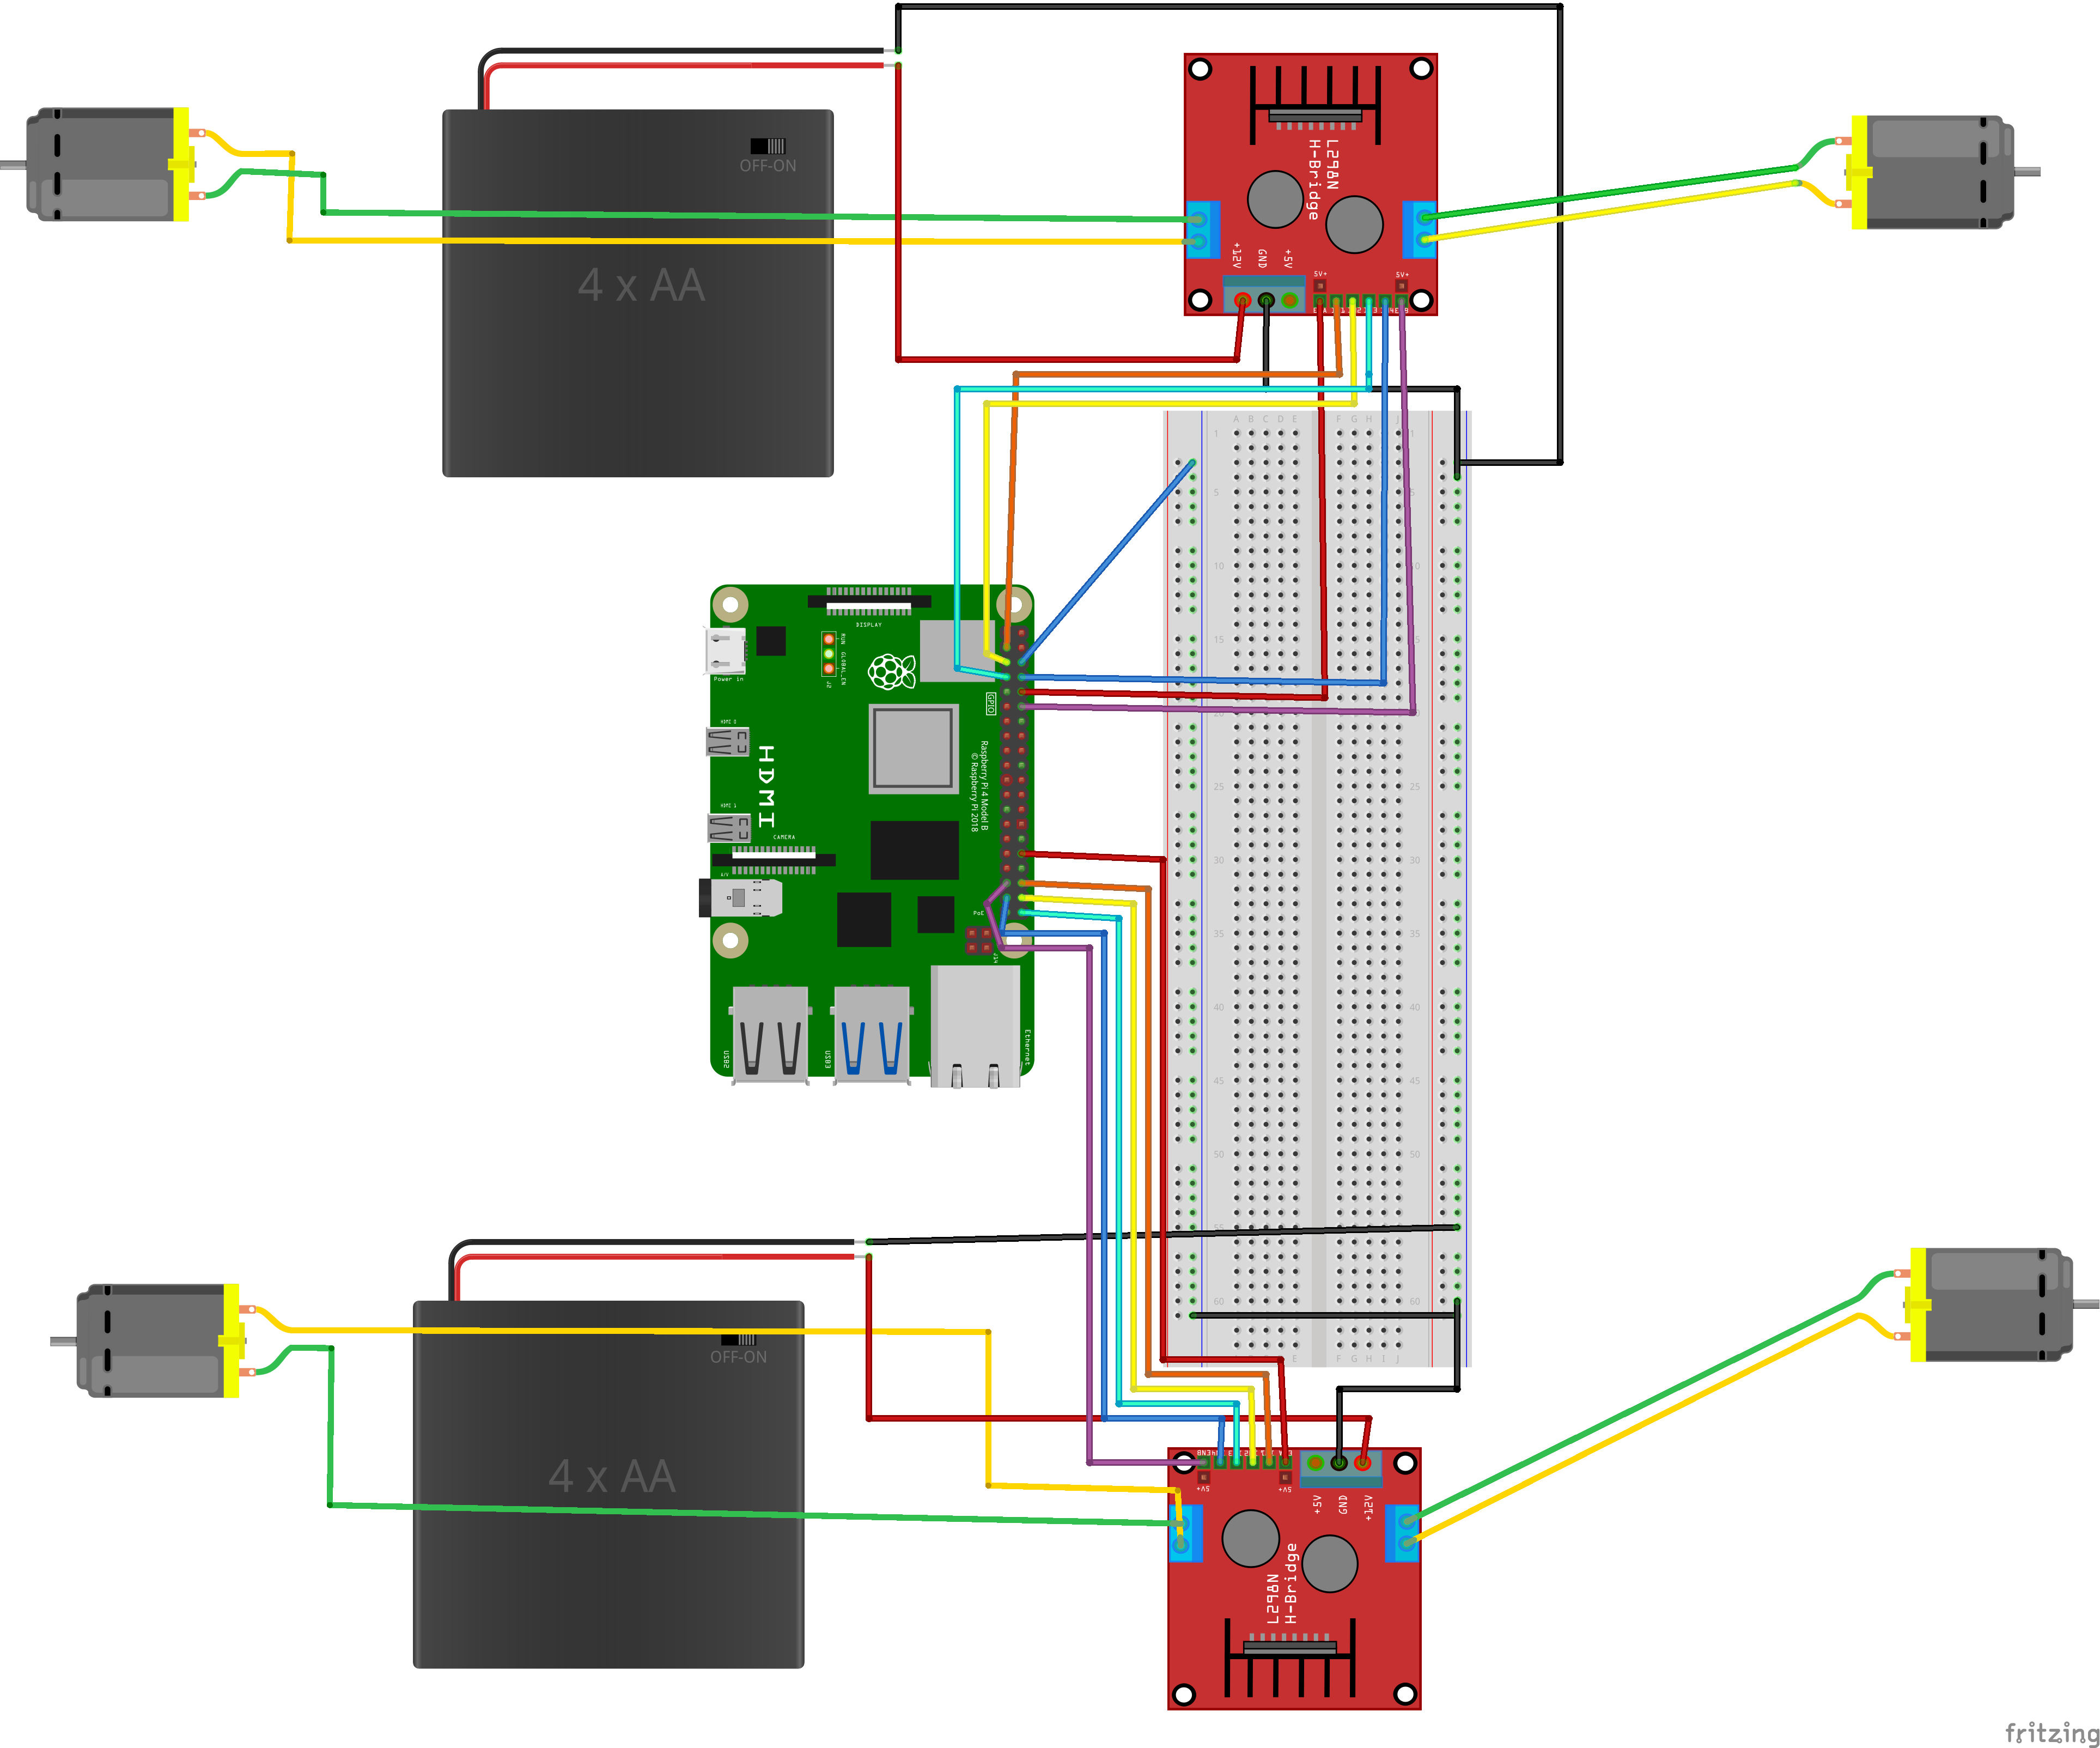
\includegraphics[width=0.5\linewidth]{imgs/motori_batterie.png}
    \caption{Circuito relativo ai motori.}
    \label{fig:enter-label}
\end{figure}
\section{Implementazione software - Raspberry}
Il server RFCOMM e il processo responsabile della gestione dei PIN GPIO sono entrambi implementati in Python. L'avvio dei due servizi è gestito tramite \texttt{systemd}, al fine di garantirne l'esecuzione automatica all'accensione del dispositivo. Il file di configurazione utilizzato per \texttt{systemd} è riportato nella sezione \textit{Artefatti e materiale utile}.
\subsection{Server RFCOMM}

Il server RFCOMM implementato espone una serie di comandi che possono essere inviati tramite connessione Bluetooth per controllare il veicolo. Le chiamate disponibili sono le seguenti:

\begin{itemize}
    \item \texttt{MOVE\_STOP}: Arresta il movimento del veicolo e attiva la luce di STOP.
    \item \texttt{MOVE\_LEFT}: Effettua una rotazione verso sinistra (le ruote sinistre si muovono in retromarcia, quelle destre in avanti).
    \item \texttt{MOVE\_RIGHT}: Comando duale a \texttt{MOVE\_LEFT}, ruota il veicolo verso destra.
    \item \texttt{MOVE\_BACK}: Attiva la retromarcia, accendendo contemporaneamente le luci di STOP e di retromarcia.
    \item \texttt{MOVE\_AHEAD}: Avvia il movimento in avanti.
    \item \texttt{TOGGLE\_TR\_LF}: Attiva o disattiva l'indicatore di direzione sinistro.
    \item \texttt{TOGGLE\_TR\_RG}: Attiva o disattiva l'indicatore di direzione destro.
    \item \texttt{TOGGLE\_HIGH\_LIGHTS}: Attiva o disattiva le luci alte.
    \item \texttt{LIGHTS\_R\_G\_B}: Imposta l'intensità dei LED anteriori nei tre canali RGB. I parametri \texttt{R}, \texttt{G} e \texttt{B} devono essere interi compresi tra 0 e 255.
    \item \texttt{SYSTEM\_SHUTDOWN}: Spegne il sistema (Raspberry Pi).
    \item \texttt{SYSTEM\_REBOOT}: Riavvia il sistema (Raspberry Pi).
\end{itemize}

\subsection{Comunicazione tra i processi}

La comunicazione tra il server RFCOMM e il processo di gestione dei GPIO avviene mediante una struttura dati condivisa, implementata come un dizionario. Il processo incaricato dell’esecuzione dei comandi effettua un controllo ciclico ogni 100ms per verificare la presenza di aggiornamenti; in caso positivo, applica le modifiche rilevate.

\section{Implementazione software – Applicazione}

L’applicazione mobile è stata sviluppata in linguaggio nativo (\texttt{Kotlin}) utilizzando l’ambiente di sviluppo Android Studio.

All’avvio, l’interfaccia mostra l’elenco dei dispositivi Bluetooth precedentemente associati. Una volta selezionato il Raspberry Pi, l’applicazione stabilisce una connessione con il server RFCOMM, consentendo l’interazione tramite la UI per l’invio dei comandi.

Tra le funzionalità implementate, è prevista la possibilità di impostare il colore delle luci anteriori tramite un selettore cromatico (color picker).

\section{Replicazione}
Per quanto riguarda la replicazione lato software, sono stati previsti due approcci distinti, in funzione del livello di competenza dell’utente: uno dedicato a utenti esperti e uno pensato per utenti meno esperti.
\newline
È opportuno sottolineare che, prima di procedere con l’implementazione software, è necessario completare la ricostruzione dell’hardware. A tal fine, si rimanda alla \textbf{Sezione 3}, che fornisce i dettagli relativi alla realizzazione fisica del dispositivo.
\subsection{Utenti esperti}

Gli utenti con maggiore esperienza possono replicare il progetto clonando il repository indicato nella \textbf{Sezione 7} e adattando gli script alle specifiche della propria installazione.

È necessario installare il servizio \texttt{macchinino.service}, disponibile nella directory \texttt{./rpi-code/systemd/}. Il file va copiato o spostato all’interno di \texttt{/etc/systemd/system/}:

\begin{verbatim}
sudo cp ./rpi-code/systemd/macchinino.service /etc/systemd/system/
\end{verbatim}

Prima dell’attivazione, è necessario modificare i riferimenti al server all’interno del file \texttt{macchinino.service}, affinché corrispondano alla configurazione della propria macchina.
\subsection{Utenti meno esperti}
Gli artefatti necessari alla replicazione del progetto sono riportati nella \textbf{Sezione 7}. Per gli utenti che non hanno familiarità con l’utilizzo di \texttt{git}, è disponibile un’immagine preconfigurata del sistema, che consente di avviare il progetto senza necessità di configurazioni manuali.
\newline
Dopo aver scaricato l’immagine del sistema, denominata \texttt{rpi-image.img.gz}, inserire una scheda SD nel dispositivo in uso. Utilizzare quindi il comando \texttt{lsblk} per individuare il nome del dispositivo corrispondente alla scheda SD (ad esempio \texttt{/dev/sdX}).

Una volta identificato correttamente il disco, eseguire il seguente comando per decomprimere e scrivere l’immagine:

\begin{verbatim}
gzip -dc rpi-image.img.gz | sudo dd of=/dev/sdX bs=4M status=progress conv=fsync
\end{verbatim}

\textbf{Attenzione}: sostituire \texttt{/dev/sdX} con il percorso corretto della propria scheda SD. L'uso errato di \texttt{dd} può comportare la perdita di dati su altri dispositivi di archiviazione.
\newline
Per facilitare l'avvio del sistema, è sufficiente creare una rete Wi-Fi utilizzando anche semplicemente uno smartphone, assegnandole il nome \texttt{macchinino} e impostando la password \texttt{macchinino1234}.

Il dispositivo si collegherà automaticamente a tale rete, dopodiché sarà possibile accedere al Raspberry Pi tramite un'applicazione come \texttt{JuiceSSH} (o un qualsiasi client SSH).

Per autenticarsi usare l'utente \texttt{macchinino} e password \texttt{macchinino1234}\footnote{\`E consigliato usare \texttt{passwd} per cambiare la password al prima accesso}.

Una volta stabilita la connessione, eseguire il seguente comando per avviare la modalità di accoppiamento Bluetooth:

\begin{verbatim}
sudo bash pair.sh
\end{verbatim}

Completata la fase di pairing, sarà sufficiente installare l’applicazione mobile realizzata per iniziare a controllare il veicolo.
\section{Artefatti e materiale utile}
Il seguente materiale potrebbe essere utili:
\begin{itemize}
    \item \href{https://github.com/romanellas24/ProjectMacchinino}{Repository Github (link)}
    \item \href{https://drive.google.com/file/d/1MoiCT64zxduojVPOSujiyetljlcGCyqI/view?usp=sharing}{Immagine del progetto (link)}
    \item \href{https://drive.google.com/file/d/1pBQub-4NPCsr4k8kCNmbKAS30iKXMzs3/view?usp=sharing}{Applicazione per il progetto (link)}
\end{itemize}
\section{Problematiche del progetto}
Le criticità riscontrate durante lo sviluppo del progetto sono principalmente riconducibili a una limitata esperienza pregressa nell’ambito della progettazione meccanica.
\newline
Una delle problematiche principali riguarda il peso complessivo del veicolo, che risulta eccessivo soprattutto quando viene montata la carrozzeria superiore. In tale configurazione, i motori installati non sono in grado di generare una coppia sufficiente per consentire le manovre di sterzata.
\newline
In assenza della carrozzeria superiore, invece, il veicolo è in grado di curvare, anche se con alcune manovre aggiuntive, risultando nel complesso funzionale.
\newline
Per ovviare a tale limitazione, si suggerisce di alleggerire ulteriormente la struttura, ad esempio utilizzando un pianale più leggero o realizzandolo interamente tramite stampa 3D, oppure adottando motori più potenti in grado di sopportare il carico attuale.

\end{document}
